\documentclass[a4paper]{scrartcl} 
\usepackage[T1]{fontenc} 
\usepackage[utf8]{inputenc} 
\usepackage[english]{babel}
\usepackage{color}
\usepackage{graphicx}
\usepackage{subfigure}
\usepackage[scaled=.90]{helvet}
\usepackage{courier}
\usepackage{float}
\usepackage[a4paper, left= 2cm, textwidth=17cm]{geometry}
\usepackage[hidelinks]{hyperref}
\makeatletter         
\def\@maketitle{
\raggedleft

\includegraphics[width = 50mm]{TULOGO.png}\\[8ex]
\begin{center}
{\Huge \bfseries \sffamily \@title }\\[4ex] 
{\Large  \@author}\\[4ex] 
\@date\\[8ex]
\end{center}}
\makeatother
\pagenumbering{gobble}
\begin{document} 

\begin{titlepage}
	\centering
	
\includegraphics[width=0.35\textwidth]{TULOGO.png}\par\vspace{1cm}
	{\scshape\Large \par}
	\vspace{1.5cm}
	{\LARGE\bfseries Course-Project-Report: Finding Dynamic Dead Writes\par}
	{\large\bfseries Program Testing and Analysis WS 2017/2018\par}
	\vspace{2cm}
	\begin{center}
	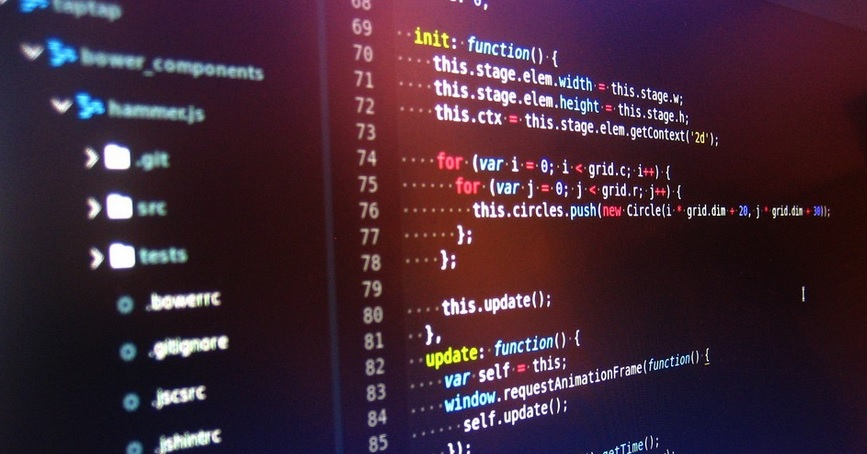
\includegraphics[width = 110mm]{Titlepage.jpg}
	\end{center}
	{\Large\itshape Kai-Nico Nase (2644914) and Nicolas Voigt (1289808)\par}
	\vfill
	supervised by\par
	Dr. Michael \textsc{Pradel}\\
	and\\
	Jibesh \textsc{Patra}	
    
	\vfill
	{\large \today\par}
\end{titlepage}

\newpage
\tableofcontents
\listoffigures% Abbildungsverzeichnis
\newpage
\pagenumbering{arabic}
\section{Abstract}
This report reflects the progress and results of a Course-Project called "Finding Dynamic Dead Writes" that is part of the subject "Program-Testing and Analysis" at TU-Darmstadt. The first part  The section "Introduction" describes in general which first steps have been taken to solve the tasks together in teamwork and which tools have been used, to simplify many things. The following sections describe then the definition of a "Dead-Write", which initial tests were carried out and of which components our project consists of. Then the approach and the implementation or components of our code analysis, which is able to detect certain types of "Dead-Writes" and afterwards cleanly remove them will be presented. Then some sample programs are listed up that contain different types of dead-writes, which our written Jalangi-Code-Analysis should be able to cleanly remove. The section results lists tasks of the task-sheet up that were performed and additional the task-results. At the end, special problems that occurred during our work on the project will be explained, as well as conclusion + outlook.
 \section{Introduction}
At the begin and after the first briefly meeting with our course-mentor, we discussed "live" first, how to configure our Test-Environment and how would be the best way to share the work, respectively "Who takes which part". Via GitHub, we set up a repository in order to keep our project-files always up to date. Due to the fact that we both live farther away from each other, we decided to hold our regular team meetings online via a free version of the Teamviewer[3] software. We also agreed at the beginning that we would like to create(for this report) diagrams or graphics with the web-based software DRAW.IO[2] so that it wouldn't be necessary to install any additional desktop-software such as e.g. MS Visio. After that, each of us installed a Linux-Image(Ubuntu) on a virtual-machine(VMWare[4]) and subsequently
the respective NodeJS[5], which is necessary to use jalangi[1] without using a web-browser. Now that we both had familiarized ourselves with Jalangi, we thought about which Callback-Functions we could use from the "Standard-Jalangi-Code-Template" to write the code analysis that Dead-Writes should find.
\subsection{Definition: What exactly are DeadWrites?}
In general, DeadWrites can be called source code elements(e.g. single or multiple statements), which have no real use during the execution of a e.g. Java-Application and are therefore superfluous. On the contrary, they can be disadvantageous and impair performance (e.g. execution speed). The simplest types of DeadWrites are simply declaring variables(e.g. var x;) that are never used again afterwards or assigning variables such as x=1; followed by y=x;. In the latter case, the value "1" is written from x to y => y=1; but y then is no longer used in a subsequent process. In the further course of this report, other DeadWrite types (Static and Dynamic) will also be presented. Static means "Write a value to a variable, but, this value is never read again afterwards and dynamically means "Write over Write", respectively, "Write" -$>$ "No Read!!!"  -$>$ "Write".
We have created eleven samples that contain one type of DeadWrite per sample. Ten are static and one dynamic.
\newpage
\section{Project consists of ...}
\subsection{... our shared repository on Github:}
\begin{figure}[!htb]
	\centering
	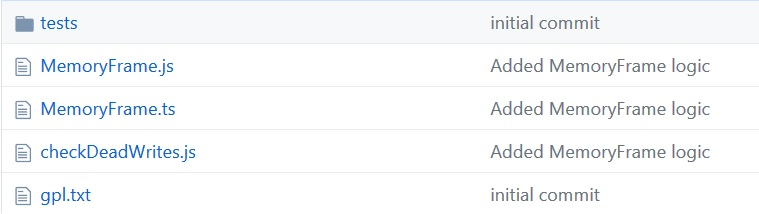
\includegraphics[width=0.6\linewidth]{Github_Content.jpg}
	\caption{Shows which files our project originally and currently consists of on "Github".}
	\label{img:grafik-dummy}
\end{figure}
\subsection{... first tests to get familar with Jalangi:}
\begin{figure}[!htb]
	\centering
	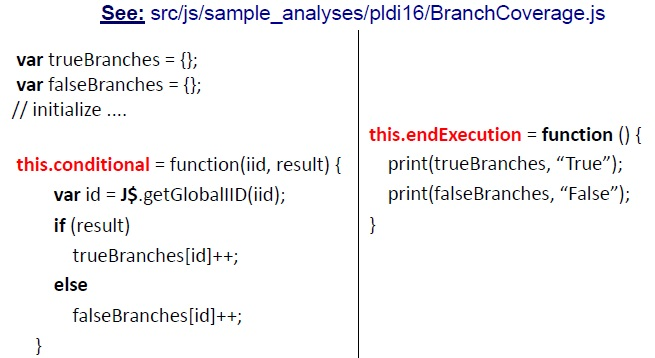
\includegraphics[width=0.8\linewidth]{FirstSampleAnalysis.jpg}
	\caption{Shows one of the first examples[6] we tried to reproduce to get more familar with jalangi, after we worked through the Jalangi standard tutorial[6]. That simple analysis counts branches which are executed of e.g a single javascript-function. After understanding how this example analysis works, we automatically had a better idea of what the term "callback function" actually means and what it does.}
	\label{img:grafik-dummy}
\end{figure}
\newpage
\subsection{... our Jalangi-Code-Analysis / Algorithm:}
The shellcommand to start our Analysis is the following:\newline "Root-Directory"/src/js/commands/jalangi.js --inlineIID -- inlineSource --analysis ./checkDeadWrites.js Level1.js\newline
Our entire code analysis consists of one Java-Script-File called "checkDeadWrites.js"(see also Figure 1).
To make things easier for us, we programmed the entire code logic  of the class, respectively, file "MemoryFrame. js" in the first step with Typescript(File "MemoryFrame.ts" on Figure 1), since type script, unlike Javascript, is a "strong typed language" and therefore offers functionalities (provided by npm) like "autocompletion" and "type-enforcing". It poses no problem from a type script file to convert a Javascript file using the shell-command "Tsc MemoryFrame.ts(creates MemoryFrame.js)" quickly and easily. In the last step we added the contents of the file "MemoryFrame.js"(in form of a Class or function called MemoryFrame only" to the end of our "checkDeadWrites.js" so that our analysis is not dependent on several files. 
All other components shown at the bottom of the diagram have been added piece by piece until the analysis has run smoothly.
The following shows the overall architecture of the components that make up our analysis:
\begin{figure}[!htb]
	\centering
	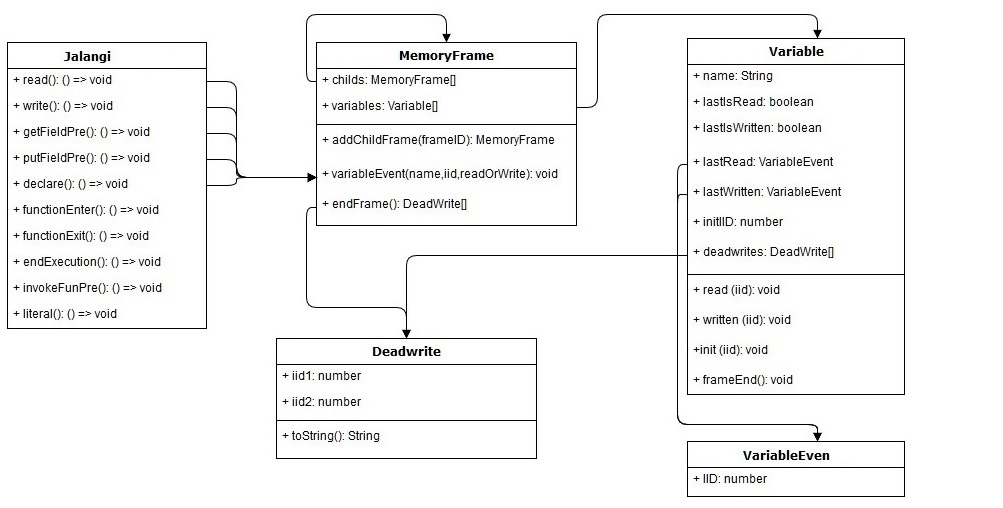
\includegraphics[width=1.1\linewidth]{WorkflowDiagram.jpg}
	\caption{Provides our code analysis algorithm or the components it consists of. The representation can be understood as a hybrid between class diagram and relationship or sequence diagram, because we also wanted to depict the sequence in which the analysis is run.}
	\label{img:grafik-dummy}
\end{figure}
\newpage
\subsection{...sampels which contains "DeadWrites"}
As already mentioned in the introduction, altogether we have created 11 different Java-Script samples, each of which contains a different type of "DeadWrite"(10 statically, 1 dynamically). The different types of DeadWrites involved were described as comments within the JS-Code-Example for each DeadWrite, below:
\begin{figure}[!htb]
	\centering
	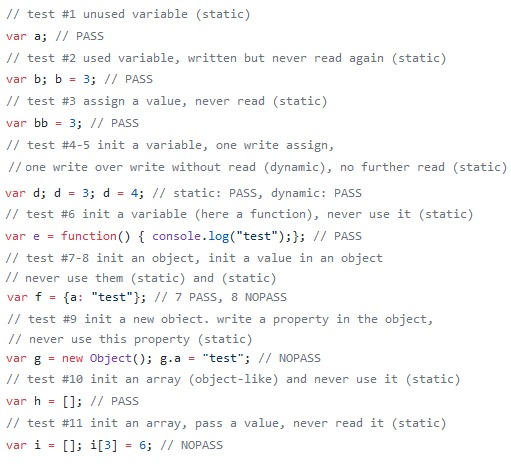
\includegraphics[width=0.5\linewidth]{Sample1.jpg}
	\caption{Shows the contents of the File "Level1.js", which  static and dynamic DeadWrites-Types our written Jalangi-Code-Analysis is able to detect. The file can be found inside the folder tests in our repository(consider Figure 1)}
	\label{img:grafik-dummy}
\end{figure}
\begin{figure}[!htb]
	\centering
	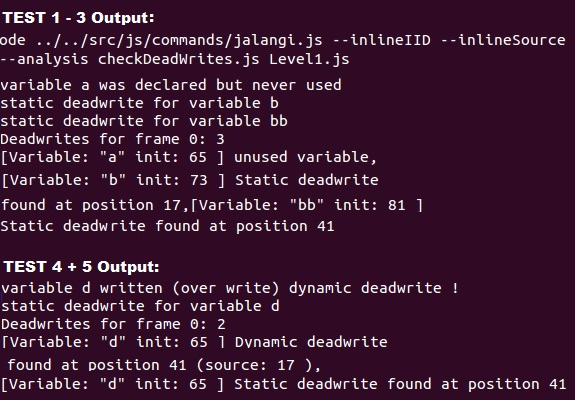
\includegraphics[width=0.5\linewidth]{OUStaticDeadWrite.jpg}
	\caption{Shows the output of Test1 - Test3 which are static DeadWrites and Test 4+5 which is static as well as dynamic.}
	\label{img:grafik-dummy}
\end{figure}
\newpage
\section{Results}
\subsection{Task performed = $\surd$ and short Result descriptions:}
\begin{enumerate}
\item Main-Goal(1): of this project is to write a Jalangi[1] analysis that will find dead writes during the execution of JavaScript programs. The analysis should guarantee that some writes are dead for some possible executions of the program. $\surd$ \newline \textit{See section Jalangi-Analysis / Algorithm}
\item Main-Goal(2): Given a JavaScript program, the output of the project will be the program without the dead writes
 $\surd$ \textit {That is performed by a launcher we have created, respectively interlinked with our J. C. analysis:} \begin{figure}[!htb]
	\centering
	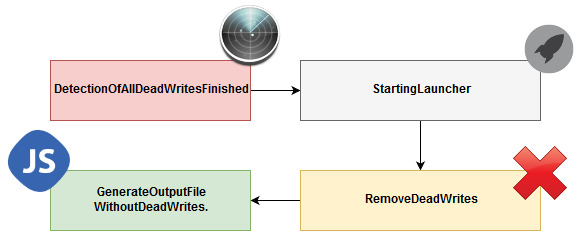
\includegraphics[width=0.6\linewidth]{Launcher.jpg}
	\caption{Shows simply the process  how to remove detected deadwrites.}
	\label{img:grafik-dummy}
\end{figure}
\item Write few simple JavaScript programs that contain dead writes  $\surd$ \newline \textit{See section samples which contain "Deadwrites"}
\item Get familiar with Jalangi2 and design and implement a Jalangi based analysis that finds dynamic dead writes  $\surd$ \textit{See section First tests + Jalangi-Analysis / Algorithm}
\item Validate your implementation with the self-written programs  $\surd$ \newline \textit{See section samples which contain "deadwrites"}
\item Parse each program using esprima to generate an AST. Traverse the AST using estraverse and delete the identify dead writes. 
\item For the final evaluation, use the JavaScript libraries Backbone, Backbone LayoutManager,BigNumber, Bootstrap Datepicker, Cal-Heatmap, Countdown, Underscore. These libraries have available tests. Run your analysis while executing these tests 
\item Remove the dead writes and run the tests again to see if any of them fail.
\end{enumerate}
\newpage
\subsection{Overall, what percentage of writes are dead?}
As can be seen in Figure 4, the analysis finds eight of eleven types of DeadWrites (PASS/NO PASS) => 8 / 11 = 72.72 $\%$.
\subsection{What is the difference in size (bytes) of the program after removing the dead writes.}
\subsection{Is there any noticeable performance improvements after removing the dead writes?}
Since we do not have the necessary equipment, we were unable to carry out such types of performance tests.
\section{Completion}
\subsection{Some Problems which occurred before or during our work}
\begin{itemize}
\item Initially it was a big challenge to familiarize our self with Jalangi. There are exists documentations and introductory examples, but from our personal point of view, they are not really easy to understand.
\item Before we could start with our work on the model or algorithm, we had to clarify beforehand, which kinds of deadwrites should be found, because this was not clearly defined on the task-sheet.
\item Programming Javascript can be very frustrating in general, because you often get little or none feedback about e.g. syntax errors or something like that.  For this reason we have pre-programmed our code logic with type script(for more infos look section "...our Jalangi Code Analysis/Alorithm)
\end{itemize}
\subsection{Conclusion + Outlook}
In this course project we've learned a lot about javascript, some of its properties and how to built a jalangi analysis that is able to detect several static and dynamic kinds of deadwrites in javascript programs. With this acquired knowledge of how to write in general a code analysis, we will also be able to use it for other purposes. The discovery of "DeadWrites" can be assigned to the area of IT security, but also to other areas. Especially for the discovery of e.g. vulnerabilities in web applications(IT-Security sector only) the acquired knowledge can be transferred in any case. As before mentioned, we will use the fundamental knowledge of what a code analysis does and how to apply it to other topics and programming languages. Once you have understood the basic principle, it is not that difficult to familiarize yourself with other code analysis frameworks, for example. One of us is particularly interested in the reverse engineering sector, where the topic of code analysis will help a lot.
\newpage
\section{References}
\mbox{-[1]- \url{https://github.com/Samsung/jalangi2}}
\newline
\mbox{-[2]- \url{http://draw.io/}}
\newline
\mbox{-[3]- \url{https://www.teamviewer.com/en/}}
\newline
\mbox{-[4]- \url{https://www.vmware.com}}
\newline
\mbox{-[5]- \url{https://nodejs.org/en/}}
\newline
\mbox{-[6]- \url{http://manu.sridharan.net/files/JalangiTutorial.pdf}}
\end{document} 

